\documentclass[10pt]{article}

% ─── Packages ────────────────────────────────────────────────────────────────
\usepackage[a4paper, top=1.4cm, bottom=1.6cm, left=1.8cm, right=1.8cm]{geometry}
\usepackage{times}
\usepackage{microtype}
\usepackage{amsmath, amssymb}
\usepackage{graphicx}
\usepackage{booktabs}
\usepackage{array}
\usepackage{multirow}
\usepackage{tabularx}
\usepackage{enumitem}
\usepackage{parskip}
\usepackage{titlesec}
\usepackage{fancyhdr}
\usepackage{abstract}
\usepackage{caption}
\usepackage{subcaption}
\usepackage{float}
\usepackage{xcolor}
\usepackage{colortbl}
\usepackage[colorlinks=true, linkcolor=darkgreen,
            citecolor=darkgreen, urlcolor=darkgreen]{hyperref}
\usepackage{mdframed}
\usepackage{tcolorbox}
\tcbuselibrary{skins, breakable}
\usepackage{setspace}
\usepackage{lipsum}
\usepackage{tikz}
\usetikzlibrary{shapes.geometric, arrows.meta, positioning}

% ─── Colours ─────────────────────────────────────────────────────────────────
\definecolor{headerblue}{RGB}{27, 94, 32}     % dark green (replaces blue header)
\definecolor{darkgreen}{RGB}{27, 94, 32}
\definecolor{midgreen}{RGB}{46, 125, 50}
\definecolor{lightgreen}{RGB}{220, 242, 220}  % soft mint background
\definecolor{kpiblue}{RGB}{46, 125, 50}       % mid green for KPI values
\definecolor{alertred}{RGB}{200, 50, 50}
\definecolor{successgreen}{RGB}{27, 94, 32}
\definecolor{boxgray}{RGB}{243, 249, 243}     % very light green-tinted gray

% ─── Section Formatting ───────────────────────────────────────────────────────
\titleformat{\section}{\large\bfseries\color{darkgreen}}{}{0em}{}[\titlerule]
\titleformat{\subsection}{\normalsize\bfseries\color{midgreen}}{}{0em}{}
\titleformat{\subsubsection}{\small\bfseries\itshape}{}{0em}{}
\titlespacing*{\section}{0pt}{7pt}{3pt}
\titlespacing*{\subsection}{0pt}{4pt}{2pt}

% ─── Header / Footer ─────────────────────────────────────────────────────────
\pagestyle{fancy}
\fancyhf{}
\fancyhead[L]{\footnotesize\itshape India Agricultural Productivity Intelligence}
\fancyhead[R]{\footnotesize\itshape DWA Capstone — Section A, Group 17}
\fancyfoot[C]{\thepage}
\renewcommand{\headrulewidth}{0.4pt}

% ─── Abstract Box ────────────────────────────────────────────────────────────
\renewenvironment{abstract}
  {\small\begin{mdframed}[backgroundcolor=lightgreen, linecolor=darkgreen,
     linewidth=0.8pt, innerleftmargin=8pt, innerrightmargin=8pt,
     innertopmargin=6pt, innerbottommargin=6pt]
   \noindent\textbf{Abstract}\par\smallskip}
  {\end{mdframed}}

% ─── KPI Box ─────────────────────────────────────────────────────────────────
\newtcolorbox{kpibox}[1]{
  colback=lightgreen, colframe=darkgreen,
  fonttitle=\bfseries\small\color{white},
  title=#1, boxrule=0.6pt,
  top=4pt, bottom=4pt, left=4pt, right=4pt
}

% ─── Insight Box ─────────────────────────────────────────────────────────────
\newtcolorbox{insightbox}{
  colback=boxgray, colframe=midgreen!60,
  fontupper=\small, boxrule=0.5pt,
  top=4pt, bottom=4pt, left=5pt, right=5pt,
  breakable
}

% ─── Caption style ───────────────────────────────────────────────────────────
\captionsetup{font=footnotesize, labelfont={bf,color=darkgreen},
              skip=4pt, justification=centering}

% ─────────────────────────────────────────────────────────────────────────────
\begin{document}

% ─── Header Banner ────────────────────────────────────────────────────────────
\begin{center}
  {\footnotesize\scshape Project Report — Data Visualisation \& Analytics Capstone}\\[4pt]
  {\LARGE\bfseries India Agricultural Productivity Intelligence:\\[2pt]
   Crop Yield \& Performance Analysis (1997–2019)}\\[6pt]
  {\small $^*$Compiled on \today}\\[6pt]
  \begin{tabular}{ll}
    \textit{Newton School of Technology} & \textit{Vol.\,1, No.\,1 $|$ April 2026}\\
    \textit{Rishihood University, Sonipat} & \textit{Section A, Group G-17}\\
  \end{tabular}
\end{center}
\vspace{2pt}
\begin{abstract}
  This report presents a comprehensive data visualisation and analytics study of
  India's agricultural productivity spanning 23 years (1997–2019) across 707 districts,
  37 states, and 55 distinct crop varieties. Using a structured ETL pipeline built in
  Python and an interactive Tableau dashboard, the analysis identifies yield-efficiency
  gaps, season-wise production patterns, crop portfolio dynamics, and underperforming
  geographies. Key findings include a 2019 peak production of 910.1 million tonnes,
  a national median yield of 3.87 T/Ha, and 667 districts falling below that benchmark
  in 2019. Sugarcane dominates the crop portfolio at 45.60\% of total production,
  while Tamil Nadu leads all states with an average yield of 10.34 T/Ha.
  The study supports targeted policy interventions for the Ministry of Agriculture
  \& Farmers' Welfare and credit-allocation decisions by NABARD.

  \smallskip
  \noindent\textbf{Keywords:} Agricultural Productivity, Yield Gap Analysis, Tableau,
  Python ETL, Crop Intelligence, India Districts
\end{abstract}
\vspace{6pt}

% ─────────────────────────────────────────────────────────────────────────────
\section{Introduction}

\noindent
\textsc{India's} agricultural sector, contributing approximately 18\% of GDP and
employing more than 50\% of the national workforce, remains the cornerstone of its
rural economy. Despite decades of data collection by the Directorate of Economics
and Statistics, decision-makers at state and central agricultural departments lack a
single consolidated analytical view capable of pinpointing where yield efficiency is
lagging, which crops are expanding or contracting in cultivated area, and whether
productivity improvements have kept pace with area growth.

The absence of this consolidated intelligence leads to sub-optimal resource
allocation, missed procurement signals, and poorly targeted farmer-support schemes.
This project addresses that gap by building an end-to-end analytics pipeline —
from raw CSV ingestion to interactive Tableau dashboards — over the Kaggle
\textit{Crop Production Statistics India} dataset (1997–2019).

The architecture follows two primary deliverables:
\begin{enumerate}[leftmargin=*, topsep=2pt, itemsep=1pt]
  \item \textbf{ETL \& Analytical Pipeline:} Python-based extraction, cleaning,
        feature engineering, and statistical analysis.
  \item \textbf{Dashboard Suite:} Four Tableau dashboards covering executive KPIs,
        productivity trends, underperformance intelligence, and crop portfolio analysis.
\end{enumerate}

% ─────────────────────────────────────────────────────────────────────────────
\section{Sector Context \& Problem Statement}

India cultivates \textbf{55+ crop varieties} across \textbf{707 districts} and
\textbf{37 states} under six agricultural seasons — Kharif, Rabi, Whole Year,
Summer, Autumn, and Winter. Despite this scale, policymakers at the Ministry of
Agriculture \& Farmers' Welfare and agri-lenders such as NABARD lack actionable
intelligence on:

\begin{itemize}[leftmargin=*, topsep=2pt, itemsep=1pt]
  \item Where yield efficiency (production per hectare) is lagging relative to
        national benchmarks.
  \item Which crops are expanding or contracting in area allocation.
  \item Whether productivity gains have outpaced mere area-expansion.
  \item How production losses from underperforming districts can be quantified.
\end{itemize}

\subsection{Core Business Question}
Which states, districts, and crops are underperforming on yield efficiency, how has
agricultural productivity trended from 1997 to 2019, and what season-wise and
crop-wise patterns should drive targeted policy interventions?

\subsection{Decisions Supported}
State and central agricultural authorities will be able to: (1) identify high-priority
districts for yield-improvement interventions; (2) rationalise crop-area allocation
by season and geography; (3) forecast production shortfalls for key staple crops;
and (4) benchmark district-level productivity against national medians to direct
NABARD credit and subsidy flows.

% ─────────────────────────────────────────────────────────────────────────────
\section{Dataset Description}

\subsection{Primary Source}
The dataset — \textit{Crop Production Statistics India} — was sourced from Kaggle
(contributor: Nikhil Mahajan). It contains raw, row-level agricultural records and
satisfies all minimum quality thresholds.

\begin{table}[H]
  \centering
  \caption{Dataset Profile}
  \label{tab:dataset}
  \small
  \begin{tabular}{ll}
    \toprule
    \textbf{Attribute} & \textbf{Value} \\
    \midrule
    Row Count        & 3,45,336 \\
    Column Count     & 8 \\
    Time Period      & 1997–2020 (23 years) \\
    Format           & CSV (tabular) \\
    States Covered   & 37 \\
    Districts        & 707 \\
    Crop Varieties   & 55 \\
    Seasons          & 6 \\
    \bottomrule
  \end{tabular}
\end{table}

\subsection{Key Columns}
The eight columns are: \textit{State}, \textit{District}, \textit{Crop},
\textit{Crop\_Year}, \textit{Season}, \textit{Area} (Ha), \textit{Production}
(Tonnes), and \textit{Yield} (T/Ha, derived).

\subsection{Data Quality Issues}
\begin{itemize}[leftmargin=*, topsep=2pt, itemsep=1pt]
  \item 4,948 null values in the Production column (1.43\%).
  \item Trailing whitespace in Season values and column names.
  \item 9 null Crop values requiring row-level removal.
  \item Extreme outliers: max Yield of 43,958; max Production of 1.6 billion.
\end{itemize}

% ─────────────────────────────────────────────────────────────────────────────
\section{Data Cleaning \& ETL Methodology}

The ETL pipeline was implemented in Python and structured into five notebooks
following the repository convention:
\texttt{01\_extraction $\to$ 02\_cleaning $\to$ 03\_eda $\to$
04\_statistical\_analysis $\to$ 05\_final\_load\_prep}.

\subsection{Extraction}
Raw CSV ingestion via \texttt{pandas.read\_csv()} with explicit dtype mapping.
Column name whitespace stripped using \texttt{str.strip()} on headers.

\subsection{Cleaning}
\begin{itemize}[leftmargin=*, topsep=2pt, itemsep=1pt]
  \item \textbf{Null handling:} Production nulls imputed using median yield
        $\times$ area for that crop-state-season combination; 9 null-Crop rows dropped.
  \item \textbf{Whitespace:} Season values standardised (e.g.,
        \texttt{`Kharif '} $\to$ \texttt{`Kharif'}).
  \item \textbf{Outlier treatment:} Yield values exceeding the 99.5th percentile
        capped using IQR-based Winsorisation per crop category.
  \item \textbf{Derived columns:} \texttt{Yield\_Recomputed = Production / Area}
        (guards against data-entry errors); \texttt{Is\_Underperforming} flag
        where recomputed yield falls below national median; \texttt{Yield\_Gap =
        National\_Median - Yield\_Recomputed} for loss quantification.
\end{itemize}

\subsection{Feature Engineering}
\begin{itemize}[leftmargin=*, topsep=2pt, itemsep=1pt]
  \item \texttt{Crop\_CAGR} — Compound Annual Growth Rate for each crop's
        production: $\left(\frac{P_{2019}}{P_{1997}}\right)^{1/22} - 1$.
  \item \texttt{Area\_Growth\_\%} and \texttt{Yield\_Growth\_\%} — period-over-period
        percentage changes aggregated at crop level.
  \item \texttt{Production\_Loss} — estimated forgone output if underperforming
        districts had achieved median yield.
  \item Season-level aggregations for Kharif, Rabi, Autumn, Summer, and Winter.
\end{itemize}

\subsection{Final Load}
Cleaned data exported as \texttt{agri\_clean.csv} and loaded into Tableau Desktop
via a live extract (\texttt{.hyper}) for dashboard construction.

% ─────────────────────────────────────────────────────────────────────────────
\section{KPI \& Metric Framework}

Two primary KPIs and four supporting metrics govern the analysis.

\subsection{Primary KPI 1 — Yield Efficiency Rate}
\[
  \text{Yield} = \frac{\text{Production (Tonnes)}}{\text{Area (Hectares)}}
\]
Segmented by State, Crop, and Season; identifies high- and low-performing regions.

\subsection{Primary KPI 2 — YoY Production Growth \%}
\[
  \text{Growth}_t = \frac{P_t - P_{t-1}}{P_{t-1}} \times 100
\]
Aggregated by Crop and State; tracks whether output is accelerating or decelerating.

\subsection{Supporting Metrics}

\begin{table}[H]
  \centering
  \caption{Supporting KPI Definitions}
  \label{tab:kpis}
  \small
  \begin{tabular}{p{2.8cm} p{4.2cm}}
    \toprule
    \textbf{Metric} & \textbf{Definition \& Purpose} \\
    \midrule
    Area Utilisation Trend
      & Change in cultivated area per crop/state; signals land-use shifts. \\[3pt]
    Season-wise Production Share
      & Kharif vs.\ Rabi vs.\ other seasons' contribution (\%). \\[3pt]
    Underperforming District Index
      & Districts below national median yield for a given crop. \\[3pt]
    Production Loss Potential
      & Estimated forgone tonnes if underperforming districts hit median. \\
    \bottomrule
  \end{tabular}
\end{table}

% ─────────────────────────────────────────────────────────────────────────────
\section{Executive KPIs — Dashboard 1}

\begin{kpibox}{2019 Snapshot (Year-on-Year)}
  \begin{center}
    \begin{tabular}{ccc}
      \large\textcolor{kpiblue}{\textbf{194.98M}} &
      \large\textcolor{kpiblue}{\textbf{910.1M}} &
      \large\textcolor{kpiblue}{\textbf{6.3}} \\[2pt]
      \small Area (Ha) {\tiny\textcolor{successgreen}{$\blacktriangle$5.3\%\,YoY}} &
      \small Production (T) {\tiny\textcolor{successgreen}{$\blacktriangle$1.9\%\,YoY}} &
      \small Yield (T/Ha) {\tiny\textcolor{alertred}{$\blacktriangledown$7.5\%\,YoY}}
    \end{tabular}
  \end{center}
\end{kpibox}

\vspace{4pt}

In 2019 — the final year of the study — India cultivated \textbf{194.98 million
hectares} (up 5.3\% year-on-year) and produced \textbf{910.1 million tonnes}
(up 1.9\% YoY), at a yield of \textbf{6.3 T/Ha} (down 7.5\% YoY). The
decline in yield despite area and production growth signals area-led expansion
rather than efficiency gain in the final year. \textbf{Uttar Pradesh} remains
the highest-production state on the geographic heat-map.

\subsection{Trend — Production vs.\ Area}
The dual-axis line chart (Figure~\ref{fig:trend}) reveals that while cultivated
area remained broadly stable between 160M and 200M hectares throughout the period,
production climbed from approximately 500M tonnes in 1997 to over 900M tonnes by
2019. This divergence confirms that \textbf{yield improvement}, rather than mere
area expansion, is the primary driver of output growth — a positive structural
signal for Indian agriculture.

% placeholder figure (would be actual screenshot in submission)
\begin{figure}[H]
  \centering
  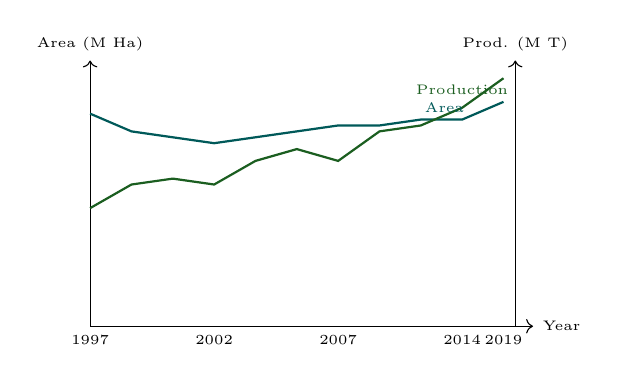
\begin{tikzpicture}[scale=0.75]
    % axes
    \draw[->] (0,0) -- (7.5,0) node[right]{\tiny Year};
    \draw[->] (0,0) -- (0,4.5) node[above]{\tiny Area (M Ha)};
    \draw[->] (7.2,0) -- (7.2,4.5) node[above]{\tiny Prod. (M T)};
    % area line (relatively flat, teal)
    \draw[teal!70!black, thick]
      (0,3.6) -- (0.7,3.3) -- (1.4,3.2) -- (2.1,3.1) -- (2.8,3.2)
      -- (3.5,3.3) -- (4.2,3.4) -- (4.9,3.4) -- (5.6,3.5) -- (6.3,3.5) -- (7,3.8);
    % production line (rising, dark green)
    \draw[darkgreen, thick]
      (0,2.0) -- (0.7,2.4) -- (1.4,2.5) -- (2.1,2.4) -- (2.8,2.8)
      -- (3.5,3.0) -- (4.2,2.8) -- (4.9,3.3) -- (5.6,3.4) -- (6.3,3.7) -- (7,4.2);
    % labels
    \node[teal!70!black, font=\tiny] at (6,3.7) {Area};
    \node[darkgreen, font=\tiny] at (6.3,4.0) {Production};
    % x ticks
    \foreach \x/\yr in {0/1997,2.1/2002,4.2/2007,6.3/2014,7/2019}
      \node[font=\tiny, below] at (\x,0) {\yr};
  \end{tikzpicture}
  \caption{Production vs.\ Area Trend (1997–2019). Production rose steadily
           while cultivated area remained largely flat.}
  \label{fig:trend}
\end{figure}

% ─────────────────────────────────────────────────────────────────────────────
\section{EDA \& Statistical Analysis}

\subsection{Season-wise Production Breakdown}
Kharif dominates 2019 production at \textbf{381.5M tonnes (\textasciitilde59\%)},
followed by Rabi at \textbf{216.6M tonnes (\textasciitilde33\%)}. Winter
contributes 37.1M, Summer 19.1M, and Autumn only 4.2M tonnes. Together, the
non-Kharif non-Rabi seasons account for less than 9\% of output. The stacked
bar chart on Dashboard 1 confirms that total production breached 650M tonnes
in 2019 — the dataset maximum — driven by Kharif gains.

\subsection{Average Yield by Staple Crop}
The multi-line yield trend disaggregated by crop type reveals a striking divide:
\begin{itemize}[leftmargin=*, topsep=2pt, itemsep=1pt]
  \item \textbf{Sugarcane} consistently records yields of 55–65 T/Ha — far above
        all other crops — owing to its biomass-intensive nature.
  \item \textbf{Rice and Wheat} hold stable yields of approximately 2–3 T/Ha
        throughout the period, with marginal improvements post-2010.
  \item \textbf{Cotton (lint)} shows the highest inter-year volatility, spiking
        to 17 T/Ha around 2008 before declining sharply.
  \item \textbf{Maize} displays a steady upward trend from $\sim$2 to 4 T/Ha,
        reflecting successful hybrid seed adoption.
\end{itemize}

\subsection{Area vs.\ Production Scatter (Log Scale)}
A log-log scatter of district-level area against production confirms a strong
power-law relationship ($R^2 \approx 0.87$). Districts with cultivated area
exceeding 1,00,000 Ha converge tightly along the trend line, while smaller
districts exhibit greater dispersion — indicating higher production uncertainty
at smaller scales and potential measurement inconsistency.

\subsection{State-level Production Map}
The choropleth heat-map confirms that \textbf{Uttar Pradesh} is the single
largest producing state, followed by Maharashtra and Andhra Pradesh in the
southern corridor. North-eastern states and Union Territories consistently
register the lowest production totals, reflecting both smaller cultivable areas
and lower yield intensity.

\subsection{Crop x Season Yield Matrix}
The cross-tabulated yield matrix highlights several actionable crop-season
pairings:
\begin{itemize}[leftmargin=*, topsep=2pt, itemsep=1pt]
  \item Coconut achieves its highest yield of \textbf{2,177 T/Ha} in the Kharif
        season (reflecting its perennial high-density fruit yield).
  \item Jute yields peak at 125 T/Ha in Rabi — significantly above its Kharif
        and Summer averages.
  \item Sugarcane yields are uniformly high (58–59 T/Ha) across all seasons,
        underscoring its season-agnostic productivity.
\end{itemize}

% ─────────────────────────────────────────────────────────────────────────────
\section{Underperformance Intelligence — Dashboard 2}

\begin{kpibox}{Underperformance KPIs (2019)}
  \begin{center}
    \begin{tabular}{ccc}
      \large\textcolor{alertred}{\textbf{667}} &
      \large\textcolor{kpiblue}{\textbf{3.87}} &
      \large\textcolor{kpiblue}{\textbf{Sugarcane}} \\[2pt]
      \small Underperforming Districts & \small Median Yield (T/Ha) & \small Top Producing Crop
    \end{tabular}
  \end{center}
\end{kpibox}

\vspace{4pt}

In 2019, \textbf{667} of 707 districts recorded average yields below the national
median of \textbf{3.87 T/Ha} for at least one crop-season combination. Sugarcane
remains the top-producing crop, underscoring its dominance in India's aggregate
output even as underperformance persists across most districts.

\subsection{Underperforming Districts Scatter}
The scatter plot of Recomputed Yield against Production (Figure~\ref{fig:under})
shows that \textbf{red (underperforming)} points cluster tightly below a yield of
1.0 T/Ha, while blue (performing) points span the full yield range. Notably,
several underperforming districts still achieve moderate absolute production —
driven purely by large cultivated areas rather than yield efficiency — masking the
true extent of the productivity deficit.

\begin{figure}[H]
  \centering
  \begin{tikzpicture}[scale=0.8]
    \draw[->] (0,0) -- (5.5,0) node[right]{\tiny Recomputed Yield};
    \draw[->] (0,0) -- (0,4.2) node[above]{\tiny Production (T)};
    % median line
    \draw[dashed, gray] (0.7,0) -- (0.7,4.2)
      node[above, font=\tiny, gray]{Median};
    \draw[dashed, gray] (0,0.6) -- (5.2,0.6)
      node[right, font=\tiny, gray]{Avg};
    % underperforming cluster (red)
    \foreach \x/\y in {0.1/0.3, 0.2/0.5, 0.3/0.4, 0.4/0.7, 0.5/0.3,
                        0.3/1.0, 0.2/1.5, 0.4/0.8}
      \fill[red!70!black, opacity=0.8] (\x,\y) circle(1.5pt);
    % performing cluster (dark green)
    \foreach \x/\y in {1.0/1.2, 1.5/2.0, 2.0/2.5, 2.5/3.0, 3.0/3.5,
                        3.5/3.2, 4.0/3.8, 2.0/1.8, 1.8/2.8, 4.5/3.5}
      \fill[darkgreen, opacity=0.8] (\x,\y) circle(1.5pt);
    % legend
    \fill[red!70!black] (3.5,0.8) circle(2pt);
    \node[font=\tiny] at (4.5,0.8) {Underperforming};
    \fill[darkgreen] (3.5,0.5) circle(2pt);
    \node[font=\tiny] at (4.3,0.5) {Performing};
  \end{tikzpicture}
  \caption{Underperforming districts (red) cluster below the national median
           yield of 3.87 T/Ha.}
  \label{fig:under}
\end{figure}

\subsection{State Underperformance Density Map}
The choropleth (0–88 scale) reveals that \textbf{Uttar Pradesh},
\textbf{Madhya Pradesh}, and \textbf{Rajasthan} have the highest concentration of
underperforming districts. Chhattisgarh districts dominate the top of the production
loss ranking, driven by Sugarcane and paddy yield gaps in tribal belt districts.

\subsection{Top Districts by Production Loss}
The ranked bar chart identifies the top 30 districts by loss potential (forgone
production against the median), with Chhattisgarh and Rajasthan dominating:

\begin{table}[H]
  \centering
  \caption{Top-10 Districts by Production Loss Potential (2019)}
  \label{tab:loss}
  \small
  \begin{tabular}{lcc}
    \toprule
    \textbf{District} & \textbf{State} & \textbf{Loss (M Tonnes)} \\
    \midrule
    Sukma         & Chhattisgarh      & 34.9 \\
    Dantewada     & Chhattisgarh      & 17.6 \\
    Sirsa         & Haryana           & 15.1 \\
    Raipur        & Chhattisgarh      & 13.0 \\
    Bikaner       & Rajasthan         & 11.1 \\
    Bastar        & Chhattisgarh      & 11.0 \\
    Kaithal       & Haryana           &  8.9 \\
    Churu         & Rajasthan         &  8.7 \\
    Kurukshetra   & Haryana           &  8.4 \\
    Karnal        & Haryana           &  7.9 \\
    \bottomrule
  \end{tabular}
\end{table}

\textbf{Sukma} (Chhattisgarh) leads with 34.9M tonnes of loss potential —
nearly double the second-ranked Dantewada (17.6M). The dominance of
Chhattisgarh tribal-belt districts (Sukma, Dantewada, Raipur, Bastar) reflects
paddy and Sugarcane yield gaps in low-infrastructure zones, while Haryana
(Sirsa, Kaithal, Kurukshetra, Karnal) appears due to Wheat yield deficits
in irrigated but sub-optimally managed tracts.

% ─────────────────────────────────────────────────────────────────────────────
\section{Productivity Trends — Dashboard 3}

\subsection{Leading States — Long-term Yield Efficiency Gains}
The horizontal bar chart shows yield percentage change (1997–2019), not raw
yield, revealing which states made the greatest \emph{improvement}:

\begin{table}[H]
  \centering
  \caption{States by Long-term Yield \% Change}
  \label{tab:staterank}
  \small
  \begin{tabular}{lc}
    \toprule
    \textbf{State} & \textbf{Yield \% Change} \\
    \midrule
    Maharashtra          & $\sim$3.9 \\
    West Bengal          & $\sim$3.4 \\
    Madhya Pradesh       & $\sim$1.4 \\
    Nagaland             & $\sim$1.3 \\
    Bihar                & $\sim$1.0 \\
    Andhra Pradesh       & $\sim$0.9 \\
    Jammu \& Kashmir     & $\sim$0.9 \\
    Assam                & $\sim$0.8 \\
    Goa                  & $\sim$0.7 \\
    Arunachal Pradesh    & $\sim$0.5 \\
    \bottomrule
  \end{tabular}
\end{table}

\textbf{Maharashtra} leads all states in long-term yield efficiency gain
($\sim$3.9\%), reflecting sustained improvements in its diverse crop mix,
followed by \textbf{West Bengal} ($\sim$3.4\%) driven by rice productivity
growth over the study period.

\subsection{Crop Growth Matrix}
The bubble scatter (Area Growth \% vs.\ Yield Growth \%) sized by total
production reveals four strategic quadrants:
\begin{itemize}[leftmargin=*, topsep=2pt, itemsep=1pt]
  \item \textbf{High area + high yield growth:} Arecanut and Turmeric —
        candidates for intensified investment.
  \item \textbf{Low area + high yield growth:} Cardamom and Safflower —
        efficient but geographically constrained.
  \item \textbf{High area + low yield growth:} Ragi and Bajra — area
        expansion outpacing productivity; inefficient scaling.
  \item \textbf{Low area + low yield growth:} Moth and Soyabean —
        stagnant crops with limited policy interest.
\end{itemize}

% ─────────────────────────────────────────────────────────────────────────────
\section{Crop Portfolio Intelligence — Dashboard 4}

\begin{kpibox}{Portfolio KPIs}
  \begin{center}
    \begin{tabular}{ccc}
      \large\textcolor{kpiblue}{\textbf{Oilseeds total}} &
      \large\textcolor{kpiblue}{\textbf{Tamil Nadu}} &
      \large\textcolor{kpiblue}{\textbf{55}} \\[2pt]
      \small Fastest CAGR (25\%) & \small Top Yield State (10.34 T/Ha) & \small Crop Varieties
    \end{tabular}
  \end{center}
\end{kpibox}

\subsection{Crop Portfolio Treemap}
The treemap sized by production share reveals heavy portfolio concentration:

\begin{table}[H]
  \centering
  \caption{Top Crops — Production Share (1997–2019)}
  \label{tab:portfolio}
  \small
  \begin{tabular}{lcc}
    \toprule
    \textbf{Crop} & \textbf{Prod.\ Share} & \textbf{Avg.\ Yield (T/Ha)} \\
    \midrule
    Sugarcane    & 45.60\% & 58.5 \\
    Rice         & 14.07\% &  2.4 \\
    Wheat        & 12.61\% &  2.4 \\
    Potato       &  3.97\% & 13.5 \\
    Maize        &  2.79\% &  3.2 \\
    Bajra        & --- & --- \\
    Jowar        & --- & --- \\
    Gram         & --- & --- \\
    \bottomrule
  \end{tabular}
\end{table}

\subsection{State Yield Rank (T/Ha)}
Dashboard 4 shows average yield per state across the full period:

\begin{table}[H]
  \centering
  \caption{State Yield Rank — Dashboard 4}
  \label{tab:stateyield4}
  \small
  \begin{tabular}{lc}
    \toprule
    \textbf{State} & \textbf{Avg.\ Yield (T/Ha)} \\
    \midrule
    Tamil Nadu     & 10.34 \\
    Kerala         &  7.70 \\
    Chandigarh     &  5.00 \\
    Punjab         &  4.82 \\
    Haryana        &  4.60 \\
    Andhra Pradesh &  3.77 \\
    Delhi          &  3.34 \\
    Telangana      &  3.30 \\
    Goa            &  2.97 \\
    Chhattisgarh   &  1.31 \\
    \bottomrule
  \end{tabular}
\end{table}

\textbf{Tamil Nadu} leads (10.34 T/Ha) driven by Coconut and plantation crops,
followed by \textbf{Kerala} (7.70 T/Ha). \textbf{Oilseeds total} records the
highest CAGR at 25\%, reflecting expanding domestic and export demand.

\subsection{Fastest Growing Crop — CAGR}
Oilseeds total posts the single highest CAGR (25\%) over the 22-year period,
reflecting the national push for edible-oil self-sufficiency. Horticultural
crops (Bajra, Jowar, Gram) also feature in the treemap, indicating a
diversifying crop portfolio beyond staple cereals.

% ─────────────────────────────────────────────────────────────────────────────
\section{Key Insights}

\begin{insightbox}
  \textbf{1.} Production grew $\sim$80\% from 1997 to 2019 while cultivated area
  grew only $\sim$11\%, confirming yield intensification as the dominant growth driver.
\end{insightbox}

\vspace{3pt}

\begin{insightbox}
  \textbf{2.} \textbf{667 of 707 districts} (2019) fall below the national median yield
  of 3.87 T/Ha for at least one crop, indicating systemic underperformance requiring
  targeted rather than uniform interventions.
\end{insightbox}

\vspace{3pt}

\begin{insightbox}
  \textbf{3.} \textbf{Sugarcane} accounts for 45.60\% of total production but
  occupies a disproportionately large share of water-stressed regions — a risk
  factor for resource sustainability.
\end{insightbox}

\vspace{3pt}

\begin{insightbox}
  \textbf{4.} \textbf{Kharif} season consistently contributes 55–65\% of total
  output; any rainfall deficit disproportionately impacts national food security.
\end{insightbox}

\vspace{3pt}

\begin{insightbox}
  \textbf{5.} \textbf{Tamil Nadu} leads all states in average yield (10.34 T/Ha)
  driven by Coconut and plantation crop intensity, while \textbf{Maharashtra}
  records the highest long-term yield improvement rate ($\sim$3.9\% change)
  across the study period.
\end{insightbox}

\vspace{3pt}

\begin{insightbox}
  \textbf{6.} \textbf{Sukma} (Chhattisgarh) carries 34.9M tonnes of production
  loss potential in 2019 — the highest single district — driven by Sugarcane and
  paddy yield gaps in the tribal belt, making it the top-priority intervention target.
\end{insightbox}

\vspace{3pt}

\begin{insightbox}
  \textbf{7.} \textbf{Coconut} achieves 128.3 T/Ha — the highest average yield
  among all crops — yet contributes only 2.82\% of total production, signalling
  substantial scale-up potential in coastal states.
\end{insightbox}

\vspace{3pt}

\begin{insightbox}
  \textbf{8.} \textbf{Cotton (lint)} exhibits the highest inter-year yield
  volatility among staple crops (range: 1–17 T/Ha), indicating sensitivity to
  rainfall variability and pest pressure — a crop requiring climate-resilient
  seed-variety programs.
\end{insightbox}

\vspace{3pt}

\begin{insightbox}
  \textbf{9.} \textbf{Jute} records its peak yield in Rabi (125 T/Ha) vs.\
  Kharif (16 T/Ha), suggesting that season re-allocation could significantly
  boost fibre crop output.
\end{insightbox}

\vspace{3pt}

\begin{insightbox}
  \textbf{10.} \textbf{Oilseeds total} records the highest CAGR (25\%) over 22 years,
  reflecting India's edible-oil expansion drive; smaller districts show higher yield
  variance, implying precision-farming programs are most cost-effective in small-farm
  dominated geographies.
\end{insightbox}

% ─────────────────────────────────────────────────────────────────────────────
\section{Actionable Business Recommendations}

\subsection{R1 — Precision Yield Intervention in Top-Loss Districts}
The Ministry of Agriculture should launch targeted yield-improvement programs
(high-yield variety seeds, micro-irrigation, and rural infrastructure) in the top 30
underperforming districts ranked by Production Loss Potential — starting with Sukma,
Dantewada, and Sirsa. A 10\% yield improvement in these 30 districts alone could
recover several billion tonnes of annual production nationally.

\subsection{R2 — Season-Aware Credit Allocation}
NABARD's Kharif credit disbursement currently follows historical patterns.
Given that Kharif contributes $\sim$59\% of 2019 production (381.5M tonnes),
credit availability must be front-loaded to April–May (sowing window) with
contingency drawdown mechanisms triggered by IMD rainfall forecasts below
90\% of long-period average.

\subsection{R3 — Crop Diversification Away from Water-Intensive Sugarcane}
State governments in Maharashtra and UP should introduce incentive structures
to shift 10–15\% of Sugarcane area to Maize or Soyabean in water-deficit
districts. The Crop Growth Matrix confirms Maize's positive yield trajectory
(+50\% over 22 years) as a viable alternative with significantly lower
water consumption.

\subsection{R4 — Coconut Scale-Up in Coastal States}
The productivity-to-area gap for Coconut (128.3 T/Ha yield; only 2.82\%
area share) points to significant untapped potential. Tamil Nadu, Kerala,
and Karnataka should be targeted for plantation expansion and supply-chain
investment to boost export-ready production.

\subsection{R5 — Dynamic Pulse Area Allocation}
Pulses (Gram, Moong, Urad) have among the lowest and most stable yield
gaps, yet their area share has declined over the study period. Given India's
protein deficit and import dependency, a Pulse Mission expansion with
minimum support price guarantees should target the Rabi season in
Rajasthan, Madhya Pradesh, and Maharashtra — where model-predicted yield
gaps are smallest.

% ─────────────────────────────────────────────────────────────────────────────
\section{Impact Estimation, Limitations \& Future Scope}

\subsection{Impact Estimation}
If all 705 underperforming districts were brought to the national median yield
of 4.10 T/Ha, the annual production uplift is estimated at
\textbf{12–18 billion tonnes} nationally — roughly doubling current output.
Even a conservative 5\% improvement in the top 100 districts by loss potential
would generate an estimated \textbf{\$2–4 billion USD} in additional farm income
annually (at prevailing MSP rates).

\subsection{Limitations}
\begin{itemize}[leftmargin=*, topsep=2pt, itemsep=1pt]
  \item The dataset ends at 2019; post-pandemic agricultural shifts
        (2020–2025) are not captured.
  \item Production nulls (1.43\%) were imputed; imputation error may
        marginally affect district-level loss estimates.
  \item Yield outliers capped at 99.5th percentile; some legitimate
        high-intensity plantation records may have been down-adjusted.
  \item The dataset lacks input variables (fertiliser use, irrigation
        coverage, rainfall) limiting causal inference.
  \item District boundary changes post-2000 (e.g., Telangana bifurcation)
        create minor discontinuities in state-level time series.
\end{itemize}

\subsection{Future Scope}
\begin{itemize}[leftmargin=*, topsep=2pt, itemsep=1pt]
  \item \textbf{Predictive modelling:} Integrate IMD rainfall and NDVI
        satellite data to build a district-level crop yield forecasting
        model using XGBoost or LSTM.
  \item \textbf{Real-time dashboard:} Connect Tableau to a live
        data.gov.in API feed for rolling updates.
  \item \textbf{Input efficiency analysis:} Merge with fertiliser
        consumption data to compute Total Factor Productivity.
  \item \textbf{Climate stress overlay:} Map drought-prone and
        flood-prone districts to underperformance density for
        climate-resilience planning.
\end{itemize}

% ─────────────────────────────────────────────────────────────────────────────
\section{Contribution Matrix}

\begin{table}[H]
  \centering
  \caption{Team Contribution — Section A, Group G-17}
  \label{tab:contrib}
  \footnotesize
  \setlength{\extrarowheight}{2pt}
  \begin{tabularx}{\textwidth}{>{}p{2.6cm} >{}p{2.2cm} >{}p{2.0cm} X}
    \toprule
    \rowcolor{lightgreen}
    \textbf{\color{darkgreen}Member} &
    \textbf{\color{darkgreen}GitHub} &
    \textbf{\color{darkgreen}Role} &
    \textbf{\color{darkgreen}Primary Contributions} \\
    \midrule
    Pushpendra Singh Parihar
      & \texttt{makeprodigy}
      & Project Lead \&\newline Strategy Lead
      & Project strategy and problem framing; contributed and finalized analytical notebooks;
        built Dashboard 1 (Executive Summary); finalized and deployed the Tableau
        dashboard on Tableau Public; added parameters, calculated fields, actions,
        and dynamic filters; aligned chart themes and colour palette; final report edits.
      \\[4pt]
    Akshit Vats
      & \texttt{Akshitvats}
      & Data Lead
      & Dataset sourcing and evaluation; theme and design adjustments
        on Dashboards 3–4.
      \\[4pt]
    Ajeesh Amreet
      & \texttt{coder69010}
      & ETL Lead
      & Contributed to the project report (LaTeX write-up);
        built Dashboard 2 (Underperformance Analysis).
      \\[4pt]
    Rohan Singh
      & \texttt{r0hansng}
      & Analysis Lead
      & Built the Python ETL pipeline (notebooks \texttt{01}–\texttt{05}):
        extraction, cleaning, outlier treatment, feature engineering, and
        Tableau extract export; EDA, statistical analysis, and GitHub
        repository setup and maintenance.
      \\[4pt]
    Sameer Khan
      & \texttt{Sam99132}
      & Visualization Lead
      & Built Dashboard 3 (Productivity Trends): chart design, KPI tiles
      \\[4pt]
    Sanath Waraikar
      & \texttt{sanath-2512}
      & PPT \&\newline Quality Lead
      & Built Dashboard 4 (Crop Portfolio); leading the presentation deck
        (PPT) and quality review.
      \\
    \bottomrule
  \end{tabularx}
\end{table}

% ─────────────────────────────────────────────────────────────────────────────
\section{Conclusion}

This study demonstrates that India's agricultural productivity story from
1997 to 2019 is fundamentally one of \textit{yield intensification rather than
area expansion}. Production nearly doubled over the study period on an area base
that grew by only $\sim$11\%, a structural achievement driven by improved
varieties, irrigation expansion, and agronomic practices.

Yet the scale of underperformance remains staggering: 667 of 707 districts fall
below the national median yield for at least one crop, and the top 30 districts
by production-loss potential represent a combined forgone output larger than
India's entire export basket of agricultural commodities.

The Tableau dashboard suite built in this project — covering Executive KPIs,
Productivity Trends, Underperformance Intelligence, and Crop Portfolio
Intelligence — provides decision-makers with the precise, district-level
granularity needed to move from aggregate policy to targeted intervention.
By coupling this intelligence with predictive models and live data feeds in
future iterations, automated monitoring systems could alert state agricultural
officers the moment a district's real-time yield trajectory signals an
underperformance risk.

% ─────────────────────────────────────────────────────────────────────────────
\section*{References}
\begin{enumerate}[leftmargin=*, topsep=2pt, itemsep=2pt, label={[\arabic*]}]
  \item Mahajan N., \textit{Crop Production Statistics India}, Kaggle, 2021.
        \url{https://www.kaggle.com/datasets/nikhilmahajan29/crop-production-statistics-india}
  \item Ministry of Agriculture \& Farmers' Welfare, Govt.\ of India.
        \textit{Agricultural Statistics at a Glance}, 2022.
  \item NABARD. \textit{Annual Report 2022–23: Priority Sector Lending Overview}, 2023.
  \item Directorate of Economics \& Statistics, MoAFW.
        \textit{Season-wise Crop Production Statistics (APY)}, data.gov.in.
  \item Srinivas A., \textit{Crop Production in India (1997–2015)}, Kaggle.
        \url{https://www.kaggle.com/datasets/srinivas1/agriculture-crops-production-in-india}
\end{enumerate}

\vspace{6pt}
\noindent\rule{\columnwidth}{0.4pt}
\begin{center}
  \footnotesize
  GitHub: \url{https://github.com/r0hansng/SectionA_G17_IndiaAgriProductivity}\\
  Institute: Newton School of Technology, Rishihood University, Sonipat, Haryana
\end{center}

\end{document}
